\chapter[Introduction]{Introduction}

\section{Space Weather}
\subsection{Definition and Impacts}
Space weather is a term used to describe the state of the space environment and
involves the influence of plasma traveling outward from the Sun and its
interaction with the heliosphere, magnetosphere, ionosphere and thermosphere
\citep{Thomson2000}. The five regions that are of primary interest of current
research include the Sun, heliosphere, magnetosphere, ionosphere and
thermosphere. In recent years, there has been interest in space weather impacts
on the outer planets as more spacecraft missions explore these regions.
At the same time, space technology is improving, and near-Earth space travel is
becoming a greater possibility. Terrestrial objects are impacted by space
weather radiation. Energetic particles can be absorbed in the metal shell of a
satellite and disrupt the function of electrical components.
Terrestrial objects affected include satellites and the space station.
Earth's surface can also be impacted by space weather; during strong
geomagnetic storms, induced ground currents can cause electrical grids to
overload and large pipeline systems may degrade faster.
\subsection{Space Weather Regions}
\begin{figure}
	\centering
	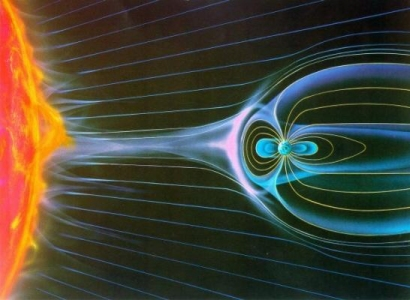
\includegraphics[scale=0.5]{images/NASA_BigPicture.jpg}
	\caption{The Sun, heliosphere, and magnetosphere (from NASA,
	\citeyear{SunHelMag}).}
    \label{fig:NASABP}
	\figSpace
\end{figure}
Figure \ref{fig:NASABP} shows a sketch of four space weather regions. The
starting point of all space weather is the Sun. The region that extends from the
solar surface to approximately 80-100 AU is called the heliosphere (the middle
region in Figure \ref{fig:NASABP} shows out to 1 AU)
\citep{Mewaldt1995}.
Inside the heliosphere are the planets, most of which have internally generated
magnetic fields that create a magnetic region known as a magnetosphere. Earth's
magnetosphere is shown on the right in Figure \ref{fig:NASABP}, its outer
boundary is defined at the location where the magnetic pressure of Earth's magnetic field
balances with the kinetic pressure of the plasma in the solar wind, and the
inner boundary is defined as the region where the exterior of Earth's
atmosphere interacts with the particles inside the magnetosphere, which is
called the ionosphere.

\subsection{Solar}
The 11-year variation in the measured solar magnetic flux and number of sunspots
defines the solar cycle \citep{Kallenrode}. All space weather originates at the
Sun, which consists mostly of fully ionized hydrogen and has a very strong magnetic field. The plasma near the
surface and the equator rotates faster than near the poles. The moving
plasma in the Sun causes its strong magnetic field \citep{Kulsrud}.

% SOLAR DYNAMO %
The solar dynamo, responsible for creating the Sun's magnetic field, is
due to the differential velocities of plasma near its surface
\citep{Kulsrud}. Differential rotation causes the magnetic field to twist and
stretch, which is defined as dynamo action. This
twisting and stretching causes increasing tensions in the solar magnetic field.
These associated poloidal and toroidal tensions cause
regions of increased surface magnetic field that appear on the solar surface as
sunspots.

% PARKER SPIRAL %
\begin{figure}
	\centering
	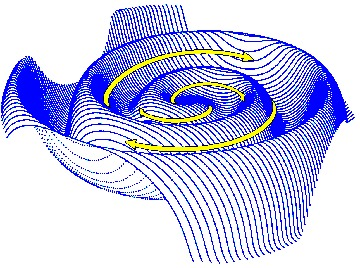
\includegraphics[scale=0.3]{images/parker.jpg}
	\caption{The Parker spiral (from NASA, \citeyear{ParkerSpiral}).}
	\label{fig:NASAParkerSpiral}
	\figSpace
\end{figure}
The twisting and stretching of the magnetic field causes the Sun to have a very
unique magnetic structure at times. Without a magnetic field, there would be a
constant flow of plasma radially outward. The presence of a magnetic field
causes changes in the location at which plasma escapes. There are different speeds of escaping plasma, and when
viewed in a cut plane of radial flow velocities in the heliosphere, a spiral
structure is expected as depicted in Figure \ref{fig:NASAParkerSpiral}.
\citet{Parker1958} first proposed the existence of this structure, now referred to 
as the Parker spiral.
% CIR %
\begin{figure}
	\centering
	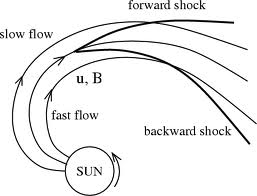
\includegraphics[scale=0.6]{images/CIR.jpeg}
	\caption{A co-rotating interaction region, (from \citeauthor{Volk2004},
	\citeyear{Volk2004}).}
	\label{fig:VolkCIR}
	\figSpace
\end{figure}
When different speeds of plasma flow outward from the Sun at different
latitudes, there are regions where fast moving plasma impacts slower moving
plasma (Figure \ref{fig:VolkCIR}) and results in a region of high density. These
regions of high density plasma are called co-rotating Interaction Regions (CIRs).

% sunspotS %
\begin{figure}
    \centering
    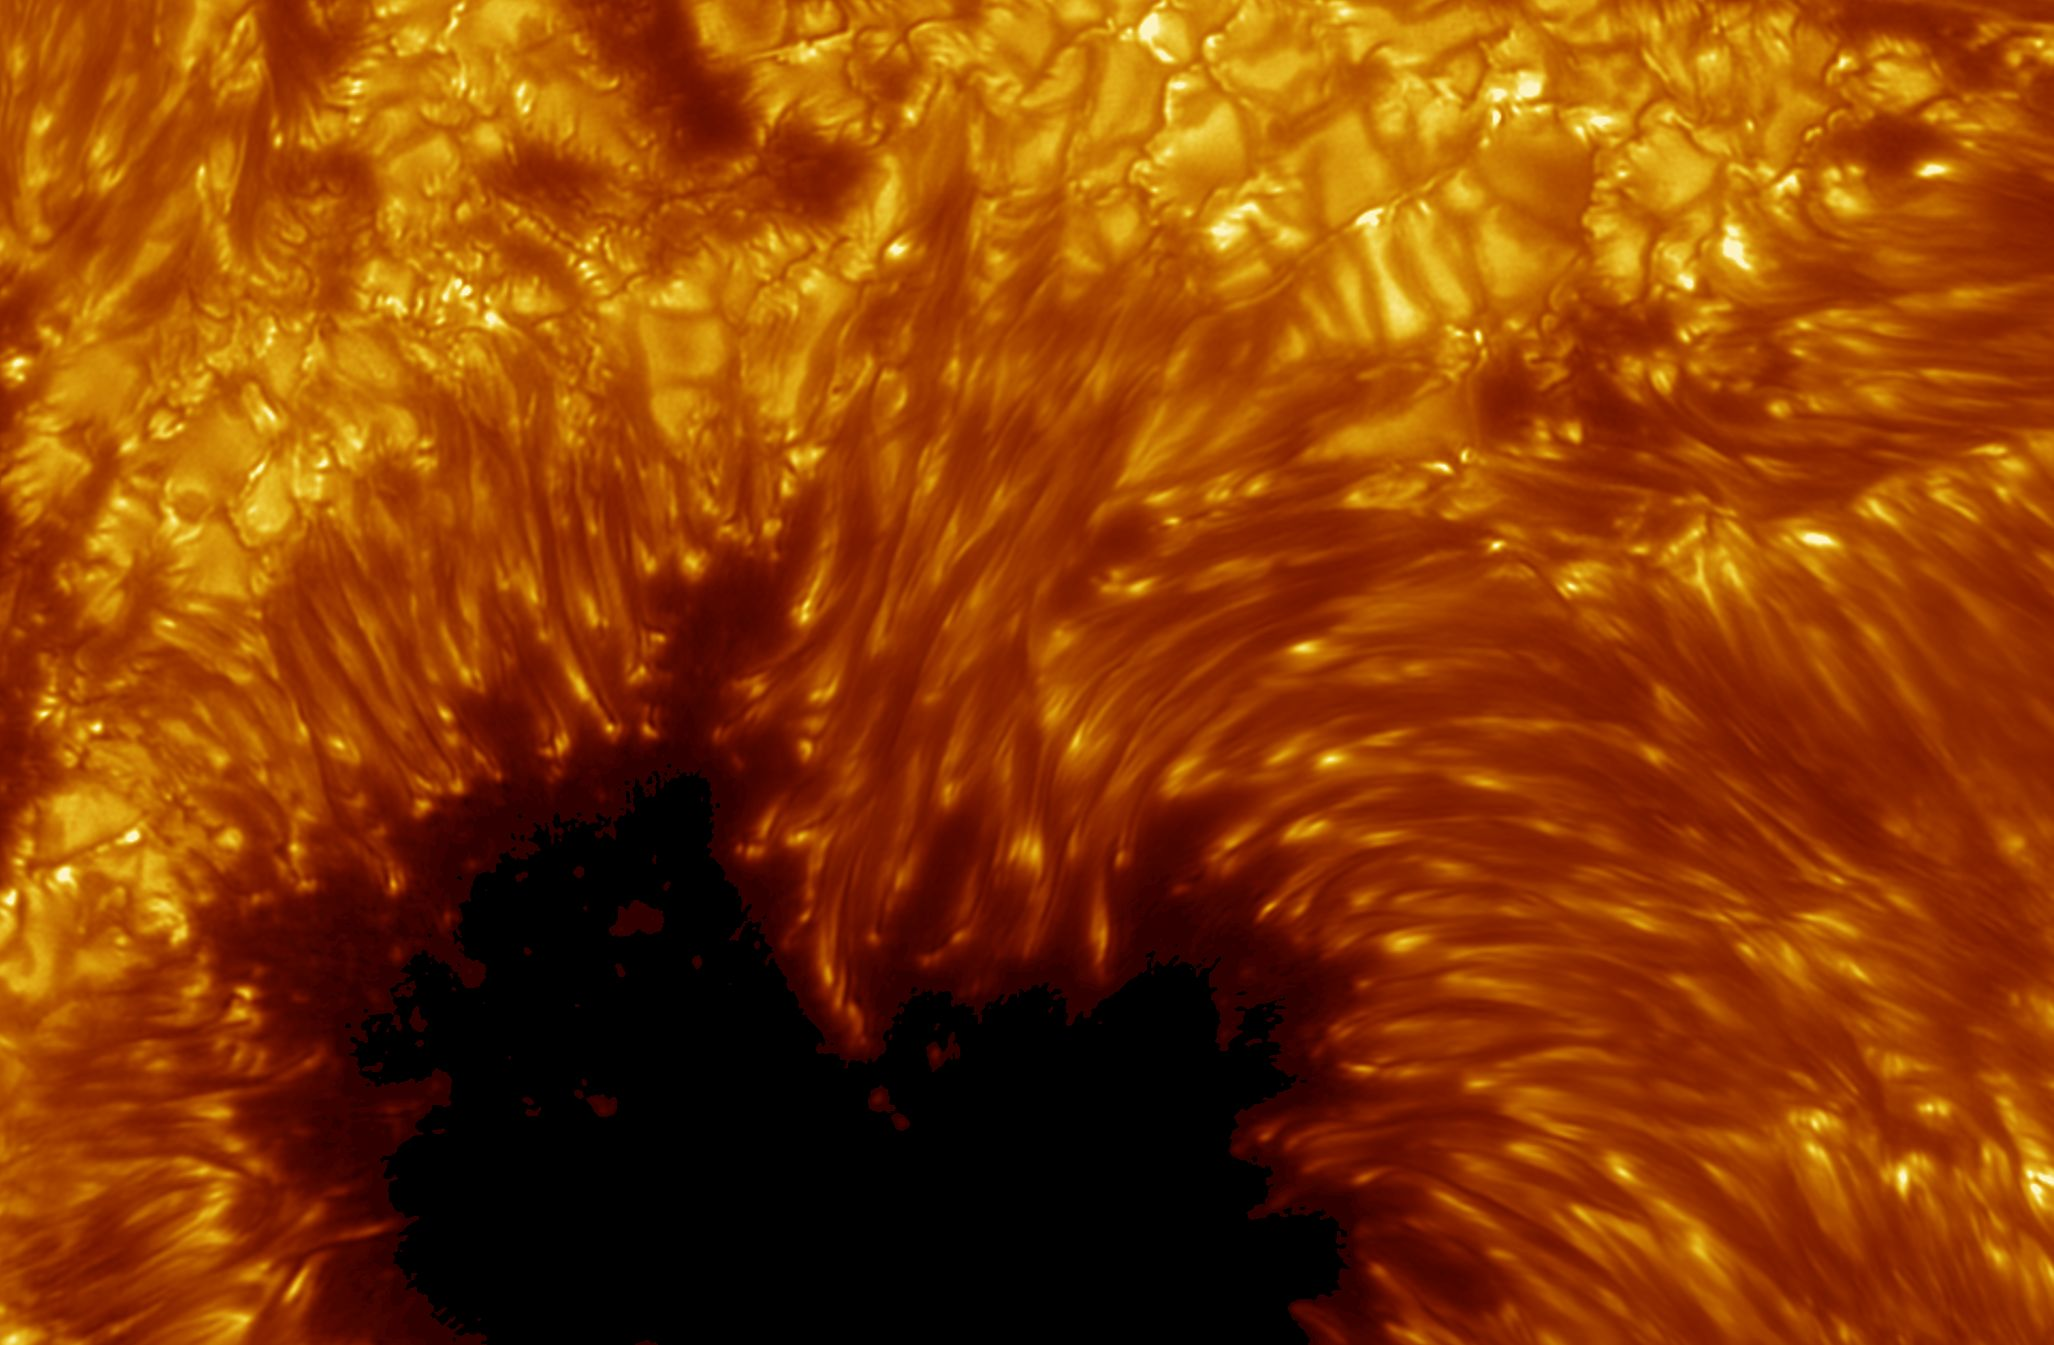
\includegraphics[scale=0.1]{images/NASA_Sunspot.jpg}\\
    \caption{A Sunspot (from NASA, \citeyear{Sunspot}).}
    \label{fig:NASAsunspot}
    \figSpace
\end{figure}
The most concern in space weather forecasting comes from events that are
associated with sunspots. Sunspots are regions of stronger magnetic field
strength on the solar surface. These regions have unique magnetic field
configurations that are believed to be related to the
cause of solar flares and Coronal Mass Ejections (CME) \citep{Kallenrode}.
Sunspots have a darker appearance as shown in Figure \ref{fig:NASAsunspot}. These regions have a
stronger magnetic field strength, giving them the darker appearance.

% SOLAR FLARES %
Solar flares are rapid bursts of energy released from the Sun. They are
typically observed as bright flashes in the visible $H_\alpha$ wavelengths.
Solar flares emit high-velocity ionized particles that can be very close to the speed of light and are used as warning signs that a CME may have occurred and could eventually be
measured by satellites near Earth (depending on their direction of
propagation).

% CME %
\begin{figure}
	\centering
	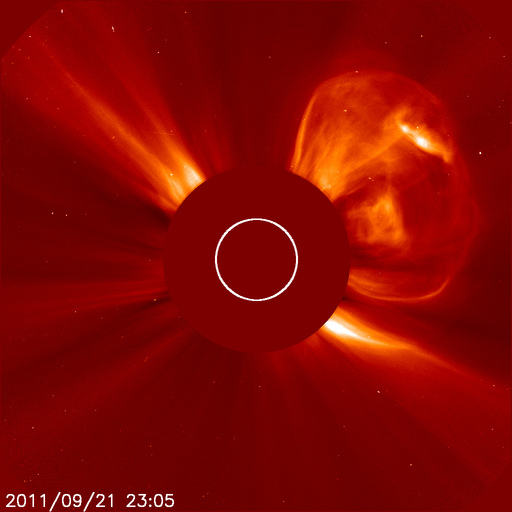
\includegraphics[scale=0.3]{images/NASA_CME.jpg}\\
	\caption{A coronal mass ejection (in the upper right corner of the image)
	taken from satellite imagery. The other two bright regions are called
	streamers (from NASA, \citeyear{CME}).}
	\label{fig:NASACME}
	\figSpace
\end{figure}
The name CME comes from satellite images showing large masses of plasma being
ejected away from the solar corona into the heliosphere, as shown in Figure
\ref{fig:NASACME}. The process that creates and drives CME	s is complex; this
process is the least understood space weather related phenomena. The plasma
associated with a CME has a shape similar to that of a light bulb and the
magnetic fields they carry are typically unorganized, complex, and difficult
to predict. Their cause is a subject of active research, but the generally
accepted explanation is that they are initiated as a result of reconnection
occurring near the sunspots \citep{Priest}.

\subsection{Heliosphere}
\begin{figure}
	\centering
	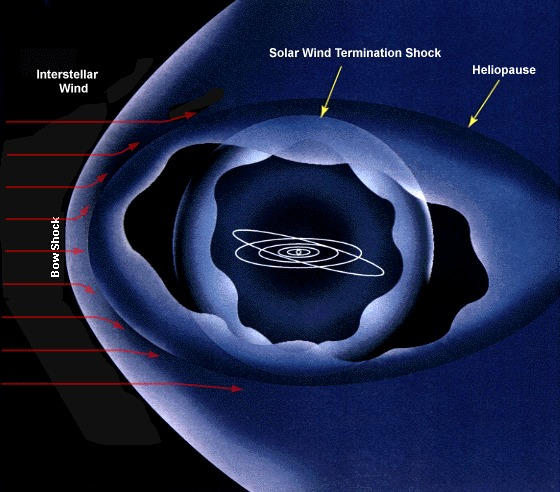
\includegraphics[scale=0.3]{images/NASA_Heliosphere.jpg}
	\caption{The heliosphere (from NASA, \citeyear{Heliosphere}).}
	\label{fig:NASAHelio}
	\figSpace
\end{figure}
The region exterior to the Sun and extending well beyond the orbit of Pluto is
called the heliosphere. Its exact shape is unknown, but an approximate tear
drop shape is depicted in Figure \ref{fig:NASAHelio}. The magnetic field it
contains decreases in strength with distance. Although the exact location of
the heliosphere boundary is unknown, it extends out well beyond the solar
system, and spacecraft have measured what is believed to be a heliopause at
approximately 120~AU \citep{Krimigis2009}. The spacecraft measurements included
a pause, sheath and shock region. These boundaries and region are explained in
detail in section \ref{MagnetosphereIntro}.

\subsection{Ionosphere/Thermosphere}
\begin{figure}
    \centering
    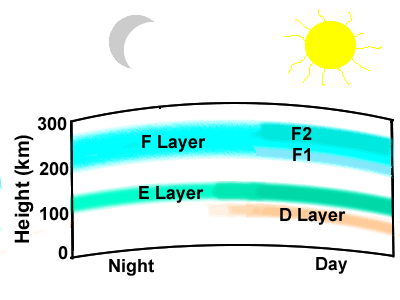
\includegraphics[scale=0.75]{images/ionosphere.png}
    \caption{The layers of Earth's ionosphere during the night time and the day
    time (from Naval Postgraduate School, \citeyear{Ionosphere}).}
    \label{fig:IonoThermo}
    \figSpace
\end{figure}
The ionosphere and thermosphere are contained within Earth's magnetosphere.
The ionosphere and thermosphere are overlapping layers that are considered
to be part of Earth's upper atmosphere, as shown in Figure \ref{fig:IonoThermo}.
The lower thermosphere boundary, which is located within the D and E regions of
the ionosphere, is defined by a rapid change in temperature, which is caused by
the absorption of ultraviolet (UV) and extreme UV (EUV) light. EUV radiation is
responsible for the creation of plasma on the sunlit side of the layer. The ionosphere has two different
profiles that are dependent on the time of day. The layers in each are labeled
as D, E, and F. The layers are defined by the density of the plasma. The F
region has the highest plasma density and is between 150-500 $km$. It is observed
more frequently in the summer time, and can separate when radiation from the
sun is highest. The E region is between 90-150 km
and the D region is below 90 km \citep{Kelley}. One importance of the ionosphere
is that high plasma densities can cause satellite drag.  Satellite drag
requires use of costly internal power resources, if available, to maintain altitude.

\subsection{Importance of Space Weather Research}
The Sun, heliosphere, magnetosphere, ionosphere, thermosphere, and all of their
phenomena are interconnected.
Understanding the thermosphere/ionosphere requires an understanding of the
magnetosphere. Understanding the magnetosphere requires an understanding of the
heliosphere. Understanding the heliosphere requires an understanding of the Sun.
As we learn more about one region, better analysis can be made in all
interconnected regions. The motivation for the pursuit of a better understanding
of space weather is due to the potential implications that adverse conditions
pose on terrestrial and space-based technology and operations.
These implications include increases in ground currents which can damage
electric power grids. HF and UHF communications can be disrupted, both of which
are vital to the air travel industry and the military. Earth-orbiting satellites
can be damaged from high energy particles. The global positioning system (GPS)
is linked to these satellites, and satellite damage could cause a loss of GPS
signals. Airplanes rely heavily on GPS. There are radiation exposure limits on astronauts
as well as humans on polar flights \citep{Pirjola2005}. The ability to
predict these adverse effects can help maintain the safety of humans in space
and ensure continual operation of space based technologies.

\subsubsection{Terrestrial Weather}
Meteorological observations in the United States have been recorded back as far
as the 17th century and were most often made along the east coast
\citep{Fiebrich2009}. Since then, significant improvements have been made. RADAR
technology used in World War 2 \citep{Page} was eventually used by the National
Weather Service (NWS). Automated Surface Observing Systems (ASOS) have been
placed throughout the country that record many meteorological conditions
\citep{Ahrens}. Today, meteorological forecasts are made and disseminated by
many sources including, but not limited to, radio stations, local television stations, the
private sector, and the government. These forecasts are made using the guidance
of forecast models. Meteorologists use the guidance of models to help make their
forecasts as accurate and precise as possible. The ability to understand all
meteorological models today would require a specific understanding of each
model. The abundance of forecasting models in the meteorology community would
make understanding each model a difficult task. With the increasing number of space weather
models, this gives motivation for improved methods for understanding forecasting
models.
\subsubsection{Space Weather}
The ability to measure space weather became possible with satellite technology.
The first satellites were launched in the late 1950s
and early 1960s \citep{Kallenrode}. In contrast to terrestrial weather, space
weather forecasts must use data that are sparse. For example, meteorology has data from ASOS to use as input data into models, which allow for the use
hundreds of input data points (ASOS, \citeyear{ASOSNum}). The sparsity of space
weather data forces forecasters to rely on numerical approximations of space
weather conditions that are not often corrected or modified by observations.
\subsubsection{Influence}
In meteorology, companies that fly airplanes or rescue teams, for example,
make decisions based on daily forecasts, and each decision has varying costs and
benefits \citep{Ahrens}. The same applies to space weather
forecasts. The companies that own and operate GPS satellites have
great interest in space weather forecasts.  For example, the airline
industry is interested in knowing whether to protect airplane
passengers by re-routing polar flights, which has varying costs and benefits
\citep{Lanzerotti2001}; \citep{Jones2005}. Finally, ground induced currents from
geomagnetic storms can effect electrical systems (GMDTF, \citeyear{GMDTF}).

\chapter{The Earth's Magnetosphere, Magnetohydrodynamics, and Magnetospheric
Models}
\section{Earth's Magnetosphere}
\label{MagnetosphereIntro}
\subsection{Discovery}
Research into the understanding of what would eventually be called the
magnetosphere started in the early 1600's when experiments were performed to
determine if garlic caused magnets to demagnetize. A similarity was found
between compass readings from a spherically shaped magnet and the direction of
mariners' compass readings. An inference was made that Earth was also a
magnet. Between the 1600's and mid-1900's there were many scientific advances in
the understanding of space weather. An important result from S.
Chapman and V. C. A. Ferraro in the early 1930's showed that solar streams were
not traveling along a direct path into Earth's upper atmosphere; they were being
deflected. Chapman and Ferraro estimated the deflection occurred at an upstream
boundary, which is known today as the Chapman-Ferraro boundary
\citep{Chapman1930}. In the 1950's, D. F. Martyn estimated the size of a
``geomagnetic hollow'' that Chapman and Ferraro predicted. This ``geomagnetic
hollow'' would eventually be named the magnetosphere by Thomas Gold in 1959.
Martyn estimated the distance to the boundary to be where the magnetic pressure
from magnetic field originating in Earth's core balanced the kinetic pressure
from a solar stream. In 1953, L. R. O. Storey researched whistlers caused from
lightning. Storey estimated that there must be plasma in the ``geomagnetic
hollow'' due to the way that Very Low Frequency (VLF) waves traveled between
Earth's hemispheres along field lines that passed through the magnetosphere.
When the U.S. and U.S.S.R. launched spacecraft to measure space weather parameters, they
found that plasma was trapped between Earth and the Chapman-Ferraro boundary,
which was not a part of the Chapman and Ferraro model of the magnetosphere
\citep{Kennel}.

\subsection{Shape}
\begin{figure}
    \centering
    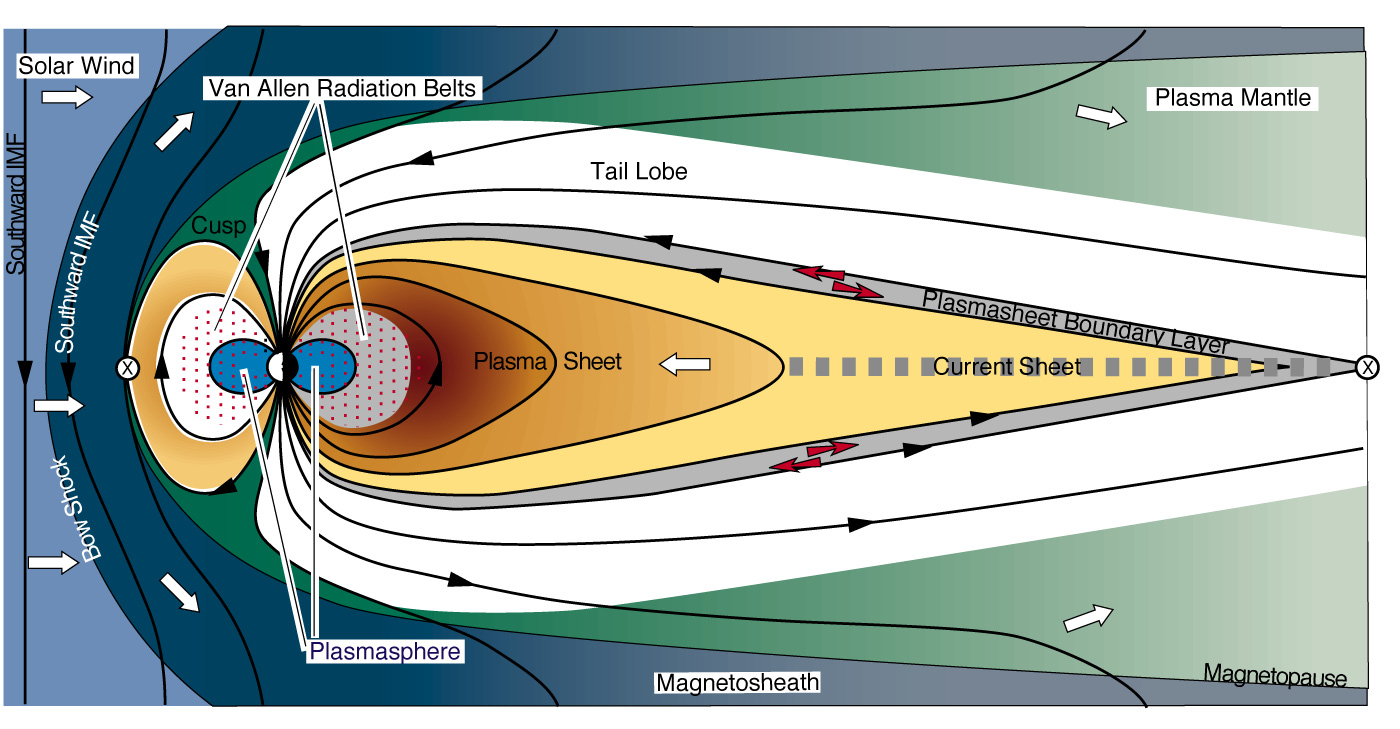
\includegraphics[scale=0.3]{images/Rice_Magnetosphere.jpg}
    \caption{The regions of Earth's magnetosphere (from Rice University,
    \citeyear{Magnetosphere}).}
    \label{fig:Rice_Magneto}
    \figSpace
\end{figure}
Based on the Chapman-Ferraro model, a calculation of the magnetopause
location could be made based on the balance between the kinetic pressure of the
solar wind and the magnetic pressure due to Earth's magnetic field. The
prediction of this model is a magnetopause at approximately 10 Earth radii
($R_E$), an overall teardrop shape, and a tail position between 50 and
100$R_E$. The processes that cause the bell shape in the magnetosphere are (1) viscosity
and reconnection and (2) change in solar wind density at the magnetopause.

\subsection{Reconnection}
Reconnection is a change in the topology of a magnetic field such that the
connectivity of field lines are changed in such a way that allows rapid conversion of
magnetic energy into kinetic energy. Reconnection is accepted to be the
source of the massive energy release associated with solar flares. Modern issues with reconnection involve questions about how such
a large amount of energy can be released in a very short amount of time.
Solar flares can release energy in the solar corona in approximately 100 seconds. Ideal
magnetohydrodynamics (MHD) can account for the time scale of energy release
but not for the amount of energy released. Non-ideal MHD accounts
for the release of a larger amount of energy but cannot match the short time
scales (Scholarpedia, \citeyear{Reconnection}). Two approaches were made to
describe how non-ideal MHD could have faster reconnection. One used a high
plasma resistivity, and the other used small dissipation scales. Sweet and Parker were the first to develop a MHD model
which had fast reconnection (by adding anomalous resistivity.) Another model was
devised by Petschek in 1964 in which the current sheet was thinner than that of
Sweet and Parker. This accounted for the small time scales and is accepted today
as the explanation for observations of fast reconnection \citep{Priest}.

\subsection{Reconnection in the Magnetosphere}
After the discovery that the solar wind was magnetized, \cite{Dungey1961}
proposed a new model of the magnetosphere that was significantly different from
the Chapman-Ferraro model.
In the Dungey model, field lines from the magnetosphere connect back into the
solar wind, as shown in Figure \ref{fig:Rice_Magneto}. The
Chapman-Ferraro model maps the fields lines between two hemispheres. Dungey's
model is considered open while the Chapman-Ferraro model is closed. Dungey's
model has two null points (shown as a white circles with an x in Figure
\ref{fig:Rice_Magneto}), which are regions where there is zero magnetic
field (and reconnection) due to the cancellation of opposing magnetic fields.
Dayside reconnection is primarily influenced by the orientation of the
interplanetary magnetic field (IMF). The magnetic field of Earth has a
northward orientation at the magnetopause. If the IMF is in the southward
direction, reconnection can occur. If the IMF direction is northward, minimal
or no reconnection occurs \citep{Priest}.

\subsubsection[The Reconnecting Magnetosphere]{The Reconnecting Magnetosphere}
\label{ReconnectingMagnetosphere}
The following section describes a long-supported view of the magnetosphere \citep{Kennel}.

\begin{figure}
	\centering
	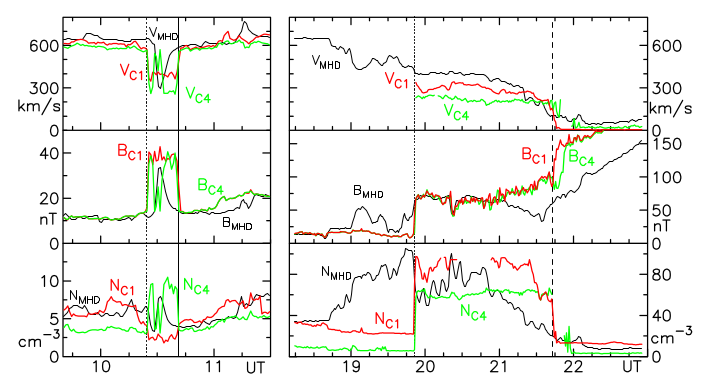
\includegraphics[scale=0.5]{images/MPandShock_VBN.png}
	\caption{Satellite measurements of velocity, magnetic field strength, and
	number density taken from Cluster 1 and Cluster 4 instruments as they
	cross through Earth's bow shock and magnetopause (from
	\citeauthor{Tatrallyay2012}, \citeyear{Tatrallyay2012}).}
    \label{fig:MPandShock_VBN}
	\figSpace
\end{figure}

\begin{figure}
	\centering
	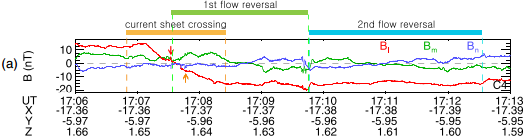
\includegraphics[scale=0.75]{images/Cur_sheet_B.png}
	\caption{Cluster 4 measurements of magnetic field strength as it crosses the
	current sheet in the magnetotail with time on the x axis; $l,m,n$
	represent current-sheet coordinates (from \citeauthor{Hwang2013},
	\citeyear{Hwang2013}).}
    \label{fig:Cur_sheet_B}
	\figSpace
\end{figure}

\begin{figure}
	\centering
	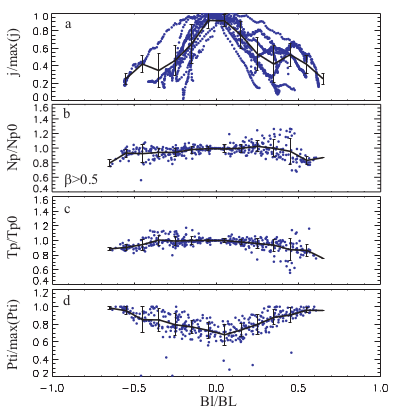
\includegraphics[scale=0.75]{images/Cur_sheet_N.png}
	\caption{Profiles of the (a) normalized current density, (b) normalized proton
	number density, (c) normalized proton temperature, (d) the sum of magnetic
	and ion pressures, versus normalized main magnetic field (from
\citeauthor{Runov2006}, \citeyear{Runov2006}).}
    \label{fig:Cur_sheet_N}
	\figSpace
\end{figure}
As shown in Figure \ref{fig:MPandShock_VBN} when passing through the bow shock
(in the Earthward direction), there is a velocity decrease, a $B$ increase at both the bow shock and magnetopause, density increase at the bow shock, and density decrease at the magnetopause.

During a magnetotail crossing, as shown in \citet{Runov2006} and
 \citet{Hwang2013}, there is a velocity increase as the distance from the
current sheet decreases. The magnetic field decreases and reverses direction as the current
sheet is crossed, as shown in Figure \ref{fig:Cur_sheet_B}. The number density
increases as the distance to the current sheet decreases, as shown in Figure
\ref{fig:Cur_sheet_N} \citep{Kennel}.

Based on many measurements similar to that described above for magnetopause and
magnetotail crossings, our general understanding of the reconnecting
magnetosphere is as follows and will be used for comparison to MHD model output
in the experiments performed:
\begin{itemize}
	\item $B_z$
	\begin{itemize}
	  \item When the $B_z^{IMF}$ is in the same direction of Earth's dipole, there
	  is a larger magnetic field strength and thus an increase in magnetic
	  pressure.
	  \item A negative $B_z^{IMF}$ and Earth's dipole oppose each
		other and decrease the magnetic pressure at the magnetopause. During these
		conditions field lines reconnect with the IMF and travel tailward.
	  \item When the magnetic pressure at the magnetopause decreases, the
	balance between the magnetic and kinetic pressures will change causing the
	magnetopause location to move Earthward.
	  \item Due to the stretching of the magnetic field tailward of Earth,
	oppositely directed magnetic field lines are moved closer causing the magnetic
	field in the current sheet region to approach zero.
	\end{itemize}
	
\item $\rho$
	\begin{itemize}
		\item As plasma travels Earthward from the Sun and encounters the magnetic
		field of Earth, it slows down. The plasma will eventually cross from
		supersonic to subsonic, creating a shock ahead of the magnetopause that is
		called the bow shock. Between the bow shock and magnetopause, plasma is
		compressed leading to higher densities.
		\item The stretching of magnetic field in the magnetotail causes oppositely
		directed magnetic field lines to become close enough to one another for
		reconnection to occur. This occurs in a plane called the current sheet and it
		separates the two opposing magnetic field directions. When reconnection occurs
		in the current sheet, a flow of new plasma replaces the plasma loss leading to
		an increase of densities. 
	\end{itemize}
	
	\item $U_x$
	\begin{itemize}
		\item The velocity of the plasma in the solar wind is supersonic. Inside the
		magnetosphere there is minimal solar wind velocity. As the
		solar wind is slows, there is a point at which it switches from supersonic to subsonic. This region is known
		as the bow shock.
		\item With the reconnection in the magnetotail occurring in the plasma sheet,
		there is a flow of plasma both towards and away from Earth on each side of
		the reconnection line. This movement is the reason that increases in
		velocities are observed as distance from the plasma sheet neutral line
		decreases.
	\end{itemize}
\end{itemize}

\subsection{Substorms}
The magnetosphere is constantly influenced by changes in the solar wind. The
direction of the IMF has the most influence. Energy from reconnection on the dayside magnetopause from a
southward IMF transfers to the magnetotail and causes a stretching of field
lines as they are dragged tailward by the solar wind. The stretching of the
field lines brings magnetic field lines of opposing direction close to one
another. Two opposing magnetic fields very close in proximity cause a sheet of
current to form. Reconnection causes a large amount of the stored
energy in the magnetotail to travel at high velocities towards Earth. The amount
of stored energy in each reconnection event is different, and so are the effects
measured at Earth. These events, as measured at Earth, are associated with substorms. On
the dayside, during times of southward IMF, the magnetopause position varies.
Many satellites have crossed the magnetopause boundary. In 1968, the OGO 5
satellite traveled towards Earth from the solar wind. The satellite recorded
approximately 10 magnetopause crossings. The first crossing was made when the
solar wind magnetic field was northward; shortly after this crossing, the
magnetic field turned southward and the satellite crossed the magnetopause once again, giving
the first measurement of the effects of southward IMF on the dayside
magnetopause. On the nightside, as the magnetopause shifts Earthward, the polar
cusps move towards the equator,	 and the thickness of the magnetotail increases
\citep{Kennel}.

\section{Magnetohydrodynamics}
\label{sec:mhd}
Magnetohydrodynamics describe the physics of magnetized fluid flow. Computational
models solve the MHD equations for a large number of points
in a specified domain.

\subsection{Single Species}
In 1872, Boltzmann derived equations that are used
today to describe the dynamics of a system that is not in thermodynamic
equilibrium. This is the starting point
for the derivation of the ideal MHD equations.
\subsubsection{Boltzman Equation}
The derivation of the single species MHD equations begins with the Boltzmann
equation for the probability distribution function
$f_s(\mathbf{x},\mathbf{v},t)$ of species s :
\begin{equation}
\frac{\partial f_s}{\partial t} + \mathbf{v} \cdot \nabla f_s + \mathbf{a}
\cdot \nabla_v f_s = \frac{\partial f_s}{\partial t}\bigg|_{coll}
\label{Boltzmann}
\end{equation}
Where $(\mathbf{x},\mathbf{v},t)$ represents position, velocity, and time,
respectively and $\mathbf{a}$ represents acceleration.
Multiplying equation \ref{Boltzmann} by a function of velocity
$\chi(\mathbf{v})$ and integrating over velocity gives:
\begin{equation}
\int \chi \frac{\partial f_s}{\partial t} d^3 \mathbf{v} + \int \chi \mathbf{v}
\cdot \nabla f_s d^3 \mathbf{v} + \int \chi \mathbf{a} \cdot \nabla_v f_s d^3
\mathbf{v} = \int \chi \frac{\partial f_s}{\partial t}\bigg|_{coll}  d^3
\mathbf{v}
\label{Boltzmann+1}
\end{equation}
This can be re-written as:
\begin{equation}
\frac{\partial}{\partial t}\int \chi f_s d^3 \mathbf{v} + \nabla \cdot \int
\mathbf{v} \chi f_s d^3 \mathbf{v} - \int f_s (\mathbf{a} \cdot
\nabla_v) \chi d^3 \mathbf{v} = \frac{\partial}{\partial t} \int \chi
f_s \bigg|_{coll} d^3 \mathbf{v}
\label{gentrans-1}
\end{equation}
where $\bigg|_{coll}$ refers to collisions between different species.

Using the definition of the average value $ < \chi >$ of a property $\chi$
of $n_s < \chi >_s = \int \chi f_s d^3 \mathbf{v}$, where $n_s$ is the number
density of species a, equation \ref{gentrans-1} becomes:
\begin{equation}
\frac{\partial}{\partial t}( n_s < \chi >_s) + \nabla \cdot (n_s < \chi
\mathbf{v} >_s) - n_s < ( \mathbf{a} \cdot \nabla_v) \chi >_s =
\frac{\partial}{\partial t} (n_s < \chi >_s)\bigg|_{coll}
\label{gentrans}
\end{equation}
which is the generalized transport equation \citep{Kominsky}.
\subsubsection{Conservation of Mass}
The law of the conservation of mass states that in a closed system the mass does
not change with time \citep{ConOfMass}. The equation for the conservation of
mass in MHD starts with equation \ref{gentrans}. For species with a mass $m_s$,
we can define:
\[ \chi = m_s \]
\[< \chi > = m_s\]
\[\mathbf{u_s} = < \mathbf{v_s} >\]
\[ \mathbf{v} = \mathbf{u_s} + \mathbf{c_s} \]
\[ < \mathbf{v_s} > = < \mathbf{u_s} + \mathbf{c_s} > \]
\[ < \mathbf{c_s} > = 0 \]
\[ < \chi\mathbf{v} >_s = m_s < \mathbf{v_s} > =  m_s \mathbf{u_s} \]
\[ \nabla_v \chi = 0 \]
Inserting these into equation \ref{gentrans} gives:
\begin{equation}
\frac{\partial}{\partial t} n_s m_s + \nabla \cdot (n_s m_s \mathbf{u_s}) = m_s
\int \frac{\partial f_s}{\partial t} \bigg|_{coll}
\label{ConOfMass-1}
\end{equation}
Defining the collision term $ S_s = \big( \frac{\partial \rho_s}{\partial t}
\big)_{coll}$, and with $\rho_s = n_s m_s$ gives:
\begin{equation}
\frac{\partial \rho_s}{\partial t} + \nabla \cdot (\rho_s \mathbf{u_s})
=  \bigg( \frac{\partial \rho_s}{\partial t} \bigg)_{coll} = S_s,
\label{ConOfMass}
\end{equation}
which is the equation for the conservation of mass \citep{Kominsky}.
\subsubsection{Conservation of Momentum}
The derivation of conservation of momentum is similar to that of mass.
Momentum cannot be created or destroyed and the amount of momentum in a specified
domain will remain constant in a closed system \citep{ConOfMomen}. Using
the property $m_s \mathbf{v}$ and defining $\chi = m_s \mathbf{v}$, equation
\ref{Boltzmann} can be written as:
\begin{equation}
\frac{\partial}{\partial t}(\rho_s < \mathbf{v} >_s) + \nabla \cdot (\rho_s <
\mathbf{v}\mathbf{v} >_s ) - n_s < (\mathbf{F_s} \cdot \nabla_v) \chi >_s = m_s
\int \mathbf{v} \bigg( \frac{\partial f_s}{\partial t} \bigg)_{coll}
\label{}
\end{equation}
Defining $\mathbf{v} = \mathbf{u}_s$ and $< \mathbf{c}_s >=0$ and solving for
$\nabla \cdot (\rho_s < \mathbf{vv} >_s)$ and $-n_s < (\mathbf{F_s} \cdot
\nabla_v) \chi >_s$ with the pressure tensor defined $P_s = \rho_s <
\mathbf{c_s c_s} >$, we arrive at the equation for the conservation of momentum \citep{Kominsky}:
\begin{equation}
\frac{\partial \rho_s \mathbf{u_s}}{\partial t} + \nabla \cdot
(\rho_s\mathbf{u_s u_s}) + \nabla \cdot (P_s) - n_s < \mathbf{F} > =
\mathbf{A_s}
\label{ConOfMomen}
\end{equation}
\subsubsection{Conservation of Energy}
The derivation of conservation of energy is similar to that of mass and
momentum. Energy cannot be created or destroyed and the amount of energy in a
specified domain will remain constant in a closed system \citep{ConOfEner}.
Starting with equation \ref{Boltzmann} and using the property $\frac{1}{2} m_s v^2$ and defining $\chi =
\frac{1}{2}m_sv^2=\frac{1}{2}m_s(\mathbf{v} \cdot \mathbf{v})$, then $\nabla_v
\chi = \frac{1}{2} m_s\nabla_v( \mathbf{v} \cdot \mathbf{v}) =
m_s(\mathbf{v}\cdot \nabla_v)\mathbf{v} = m_s\mathbf{v}$ gives:
\begin{equation}
\sum_s \frac{\partial}{\partial t} (\frac{1}{2}\rho_s < v^2 >_s) + \sum_s \nabla
\cdot (\frac{1}{2}\rho_s <v^2 \mathbf{v} >_s) - \sum_s n_s < \mathbf{F} \cdot
\mathbf{v} >_s = \frac{\partial}{\partial t}(\frac{1}{2} \rho_s < v^2
>_s)\bigg|_{coll}
\end{equation}
Solving for $\nabla \cdot (n_s < \chi \mathbf{v} >_s)$ , $- n_s < \mathbf{a}
\cdot \nabla_v \chi >_s$, and $< \mathbf{F} \cdot \mathbf{c_s} >$, this gives
an equation for conservation of energy:
\begin{equation}
\frac{\partial \epsilon_s}{\partial t} + \nabla \cdot (\epsilon_s \mathbf{u}_s)
+ \nabla \cdot (P_s \cdot \mathbf{u}_s) + \nabla \cdot \mathbf{q}_s -
n_sq_s\mathbf{u}_s \cdot \mathbf{E} - \rho_s\mathbf{u}_s \cdot \mathbf{g} = M_s
\label{ConOfEner}
\end{equation}
where $$\epsilon_s = \frac{p_s}{\gamma - 1} + \frac{1}{2} \rho_s u^2_s $$
$$P_s = \frac{1}{d} \sum_{ij} P_{aij}\delta_{ij} = \frac{1}{d}\sum_i P_{aii}$$
 $$\mathbf{q}_s = \frac{1}{2}\rho_s <c^2_s \mathbf{c}_s >$$
\subsection{Single Fluid}
The previous equations are applicable to each species in a plasma. To
allow for the treatment of the fluid as a whole, the individual species can be
summed. The following properties are defined by a sum over all species.
$$ \rho = \sum_s n_s m_s $$
$$ \rho \mathbf{u} = \sum_s n_s m_s \mathbf{u}_s $$
$$ \rho_q = \sum_s n_s q_s $$
$$ \mathbf{J} = \sum_s n_s q_s \mathbf{u}_s $$
\subsubsection{Conservation of Mass}
Using the above summations, equation \ref{ConOfMass} becomes:
\begin{equation}
\frac{\partial\rho}{\partial t} + \nabla \cdot (\rho \mathbf{u}) = 0
\label{FluidConOfMass}
\end{equation} 
\subsubsection{Conservation of Momentum}
Using the above summations, equation \ref{ConOfMomen} becomes:
$$ \sum_s \frac{\partial \rho_s \mathbf{u}_s}{\partial t} + \sum_s \nabla \cdot
(\rho_s \mathbf{u}_s \mathbf{u}_s) + \sum_s \nabla \cdot (P_s) - \sum_s
n_s(q_s(\mathbf{E} + \mathbf{u}_s \times \mathbf{B}) + m_s\mathbf{g}) = \sum_s
\mathbf{A}_s $$
Because the sum of the collision terms is zero, and total momentum is
conserved, the previous equation can be written as:
$$\frac{\partial \rho \mathbf{u}}{\partial t} + \nabla \cdot \sum_s \rho_s
\mathbf{u}_s \mathbf{u}_s + \nabla \cdot \sum_s P_s - \rho_q\mathbf{E} -
\mathbf{J} \times \mathbf{B} - \rho \mathbf{g} = 0 $$
Solving for the summations results in an equation for the conservation of
momentum for a single fluid:
\begin{equation}
\frac{\partial \rho \mathbf{u}}{\partial t} + \nabla \cdot (\rho
\mathbf{u u}) + \nabla \cdot P - \rho_q\mathbf{E} - \mathbf{J}
\times \mathbf{B} - \rho \mathbf{g} = 0
\label{FluidConOfMomen}
\end{equation}
\subsubsection{Conservation of Energy}
Using the above summations, equation \ref{ConOfEner} becomes:
$$ \sum_s \frac{\partial \epsilon_s}{\partial t} + \sum_s \nabla \cdot
(\epsilon_s \mathbf{u}_s + P_s \cdot \mathbf{u}_s + \mathbf{q}_s) - \sum_s n_s
q_s \mathbf{u}_s \cdot \mathbf{E} - \sum_s \rho_s \mathbf{u}_s \cdot \mathbf{g}
= 0 $$
Upon solving for $ \sum \rho_s u_s^2 $, $\sum_s \epsilon_s $, and $\sum_s p_s
\mathbf{u_s} $, where the total scalar pressure is
$$p = \frac{1}{d} \sum_i P_{ii} = \frac{\gamma - 1}{2} \sum_s \rho_s < ( c_s
+ w_s)^2 > = \sum_s p_s + \frac{\gamma -1}{2} \sum_s \rho_s w_s^2,$$
and the total heat flux is
$$ \mathbf{q} = \frac{1}{2} \sum_s \rho_s < (c_s + w_s)^2(\mathbf{c}_s +
\mathbf{w}_s) > ,$$
this gives conservation of energy:
\begin{equation}
\frac{\partial \epsilon}{\partial t} + \nabla \cdot (\epsilon \mathbf{u} + P
\cdot \mathbf{u} + \mathbf{q}) - \mathbf{J} \cdot \mathbf{E} - \rho\mathbf{u}
\cdot \mathbf{g} = 0.
\label{FluidConOfEner}
\end{equation}
\subsubsection{Maxwell's Equations}
Maxwell's equations relate $\mathbf{E}$, $\mathbf{J}$, and $\mathbf{B}$ from the
previous plasma equations:
\\Gauss's law:$$ \nabla \cdot \mathbf{E} = \frac{\rho_q}{\epsilon_0}$$
Gauss's law for magnetism: $$ \nabla \cdot \mathbf{B} = 0 $$
Faraday's law:$$ \nabla \times \mathbf{E} = - \frac{\partial
\mathbf{B}}{\partial t} $$ 
Ampere's law:$$ \nabla \times \mathbf{B} = \mu_0(\mathbf{J} + \epsilon_0
\frac{\partial \mathbf{E}}{\partial t}) ,$$
where $\mu_0$ is the permeability, $\epsilon_0$ is the permittivity,
$\mathbf{E}$ is the electric field, $\mathbf{B}$ is the magnetic field,
$\mathbf{J}$ is the current, and $\rho_q$ is the charge density.
\subsubsection{Conservation of Current Density}
Using Maxwell's equations, the single species momentum
equation multiplied by $\frac{q_s}{m_s}$ and summed over species
gives:
$$ \frac{\partial}{\partial t} \sum_s n_s q_s \mathbf{u}_s + \nabla \cdot
(\sum_s n_s q_s \mathbf{u}_s \mathbf{u}_s) + \nabla \cdot (\sum_s
\frac{q_s}{m_s} P_s) - \sum_s n_s \frac{q_s}{m_s} < \mathbf{F} > = \sum_s
\frac{q_s}{m_s} \mathbf{A}_s$$ Noting that:
$$ \mathbf{J} = \sum_s n_s q_s \mathbf{u}_s $$
gives conservation of current density:
\begin{equation}
\frac{\partial \mathbf{J}}{\partial t} + \nabla \cdot (\mathbf{J u} + \mathbf{u J} 
- \rho_q \mathbf{uu} + \mathbf{P}_q) - \sum_s n_s \frac{q_s}{m_s} < \mathbf{F}
> = \sum_s \frac{q_s}{m_s} \mathbf{A}_s
\end{equation}

\subsection{Ideal}
To simplify the single fluid MHD equations, the following
assumptions are made:
\begin{itemize}
\item The time derivative of E is small.
\item Isotropic Pressure: \\
If the pressure tensor $P$ is replaced with $p\mathbf{I}$, then $\nabla \cdot P
= \nabla p$.
\item Charge neutrality: $\rho_q = 0$.
\item Neglect small terms: \\
Terms involving $P_q$ can be neglected if $p_e$ is small.
\item Single ion flow with collision term approximation: \\
Used to simplify the magnetic field differential equation.
\item Perfect conductivity: \\
$\sigma$ is infinite so that $\mathbf{E} + \mathbf{u} \times \mathbf{B} =
\frac{\mathbf{J}}{\sigma} \simeq 0$, giving $\mathbf{E} = - \mathbf{u} \times
\mathbf{B}$
\end{itemize}

Using these assumptions along with Maxwell's equations, the conservation equations become \citep{Kominsky}:
\begin{itemize}
  \item Conservation of Mass
  $$ \frac{\partial \rho}{\partial t} + \nabla \cdot (\rho \mathbf{u}) = 0$$
  \item Conservation of Momentum
  $$ \frac{\partial \rho \mathbf{u}}{\partial t} + \nabla \cdot \left[\rho
  \mathbf{uu} + (p + \frac{B^2}{2\mu_0})\mathbf{I} - \frac{1}{\mu_0}
  \mathbf{BB}\right]- \rho \mathbf{g} = 0$$
  \item Conservation of Energy
  $$ \frac{\partial \epsilon}{\partial t} + \nabla \cdot \left[( \epsilon + p +
  \frac{B^2}{2\mu_0})\mathbf{u} + \mathbf{q} - \frac{1}{\mu_0}(\mathbf{u} \cdot
  \mathbf{B}) \mathbf{B}\right] - \rho \mathbf{u} \cdot \mathbf{g} = 0 $$
  \item Conservation of Magnetic Flux
  $$ \frac{\partial \mathbf{B}}{\partial t} + \nabla \cdot (\mathbf{uB} - \mathbf{Bu}) = 0 $$
\end{itemize}

\section{Magnetospheric Models}
To most accurately model the magnetosphere, the collisionless Boltzmann equations for individual species
along with Maxwell's equations should be used. The use of these equations in a
computational model is costly because the computational complexity of the
algorithms for their solutions are high \citep{Raeder2003}. A more efficient solution is
to use the ideal MHD equations. In the magnetospheric community, there are three
often-used models that implement ideal MHD. The way that each magnetospheric
model approaches these equations gives them their uniqueness.

\subsection{Grid and Geometry}
Each model uses a choice of a numerical grid and numerical method to solve the MHD equations. For the
magnetosphere, Earth's magnetopause can expand to tens of Earth radii
towards the Sun, so the simulation domain for the grid must be at least this large.
The tailward boundary can be $\ge$ 200 $R_E$, and the transverse regions are
typically $\ge$ 50 $R_E$. The choice for the numerical grid resolution and size
depends on the computational resources; the grid choice is also influenced by
the numerical method. Grids used in MHD models include:
\begin{itemize}
  \item Uniform Cartesian \\
  \begin{figure}
  	\begin{centering}
  	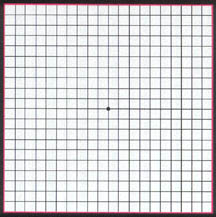
\includegraphics[]{images/UniformCartesian.jpg}
  	\caption{Uniform Cartesian Grid (from StackOverflow, \citeyear{UnifCart}).}
  	\label{fig:UniformCartesian}
  	\end{centering}
  	\figSpace
  \end{figure}
  Uniform grids as shown in Figure \ref{fig:UniformCartesian} have equal spacing
  in all dimensions.
  The amount of programming required and the computational resources used are low, and parallelization is the most straightforward to implement. The most significant limitation of the uniform cartesian
  grids is that the same resolution must be used everywhere in the domain. The optimal
  resolution is not necessarily the same for all regions of the domain.
  
  \item Stretched Cartesian \\
  \begin{figure}
  	\begin{centering}
  	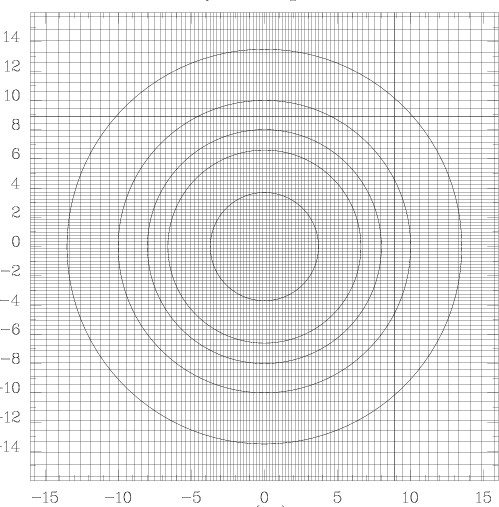
\includegraphics[scale=0.45]{images/StretchedCartesian.jpg}
  	\caption{Stretched Cartesian Grid (from Univeristy of New Hampshire,
  	\citeyear{StretchCart}).}
  	\label{fig:StretchedCartesian}
  	\end{centering}
  	\figSpace
  \end{figure}
  Stretch Cartesian grids, as shown in Figure \ref{fig:StretchedCartesian}, can
  be ``stretched'' in each dimension while still maintaining the ease of
  programming comparable to a uniform cartesian grid. The stretching can allow
  for higher resolution in regions around Earth, magnetopause, and bow
  shock regions, and other regions where needed, and lower resolution in areas
  that do not need it such as the distant magnetotail. Specifically for the
  magnetosphere, this grid type is very well adapted.
  
  \item Structured Adaptive Mesh Refinement (SAMR) \\
  \begin{figure}
  	\begin{centering}
  	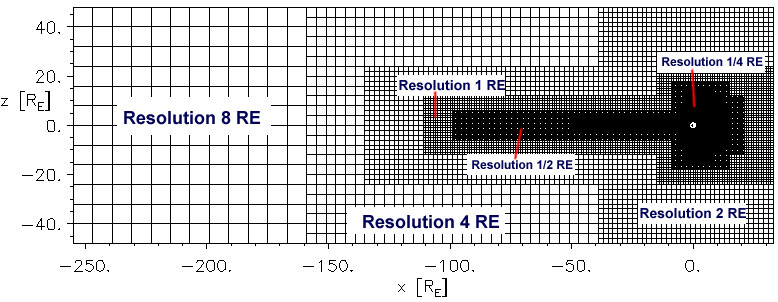
\includegraphics[scale=0.45]{images/SAMR.JPG}
  	\caption{Structured Adaptive Mesh Refinement Grid (from NASA,
  	\citeyear{SAMR}).}
  	\label{fig:SAMR}
  	\end{centering}
  	\figSpace
  \end{figure}
  SAMR grids, similar to that shown in Figure \ref{fig:SAMR}, have higher
  grid resolutions in regions that need it. These higher resolutions are
  added and removed as time progresses as needed. Different
  refinements are possible, which requires a larger coding and computational
  resource cost, yet SAMR can provide the
  most accurate solutions \citep{Raeder2003}.
  
  \item Unstructured Grid \\
  \begin{figure}
  	\begin{centering}
  	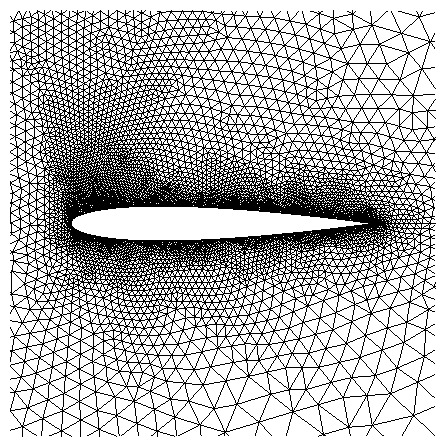
\includegraphics[scale=0.45]{images/Unstructured.jpg}
  	\caption{Unstructured Grid (from Delft University of Technology,
  	\citeyear{Unstruc}).}
  	\label{fig:Unstructured}
  	\end{centering}
  	\figSpace
  \end{figure}
  In an unstructured grid, as shown in Figure \ref{fig:Unstructured}, the shape
  of each cell is typically different than its neighbors. These grids are
  typically used in finite element and finite volume methods. They are very
  difficult to program, computationally expensive, and are difficult to
  parallelize. Their major benefit is the ability to form well to the object
  they model.
\end{itemize}

\subsection{Boundary Conditions}
On the sunward side of the grid boundary, the boundary conditions can be fixed
or time dependent. As solar wind data is measured at only a few points
near the boundary, it is difficult to determine the extended structure of the
solar wind boundary conditions. On all other boundaries, free flow conditions apply
with the exception that the $\nabla \cdot \mathbf{B} = 0$ condition is used to derive the
normal of the magnetic field (and should be consistent with the numerical
scheme) \citep{Raeder2003}.

\subsection{Initial Conditions}
\label{InitialConditions}
On the sunward side of Earth, there is a region where its magnetic field
reaches near zero. The initial conditions for $B$ are created by placing a
mirror dipole sunward of Earth such that a plane with zero magnetic field exists
close to Earth on the sunward side.
The initial solar wind and magnetic field then replaces the mirror dipole
sunward of the near zero B region.
The plasma initial conditions are typically set at a temperature of
$5000$ [$^\circ$K] and a density of $0.1$ [$cm^{-3}$]. With these initial
conditions, it can take up to ond hour for the magnetosphere to start forming. Because
the magnetosphere has a memory of previous conditions that can last
many hours, it is important to allow at least a few hours of preconditioning
time before using input data for a specific event \citep{Raeder2003}. To date,
no evaluation of the influence of preconditioning on model results has been
published.

\subsection{Spatial Discretization}
There are four different approaches used for spatial discretization in MHD
models of the magnetosphere: finite differences, finite volumes, finite
elements, and spectral.

Finite difference methods are most used in magnetospheric models, and some of
the concepts from finite differencing schemes are found in the other methods.
Conservative finite difference schemes have the best fit for global MHD
simulations \citep{Raeder2003}.

\subsection{Numerical Implementation}
There are simple differencing schemes that can have 2nd order accuracy.
Schemes such as predictor-corrector and leap-frog can be accurate,
but they lack stability, which is required in a majority of the computational
domain. The Courant-Friedricks-Levy (CFL) criteria limits the timestep for
stability. The Alfv\'en speed can be extremely large. A ``Boris Correction" or
some variant is used to limit the Alfv\'en speed allowing for larger time steps
without increasing errors in the solution \citep{Raeder2003}.

\subsection{The Open Global Geospace Circulation Model}
The Open Global Geospace Circulation Model (OpenGGCM) solves the ideal MHD
equations for the magnetosphere using a conservative finite
difference method for the gas dynamic part of the normalized ideal MHD equations.
The equations solved are: $$ \frac{\partial \rho}{\partial t} = -\nabla \cdot
(\rho \mathbf{v}) $$ $$ \frac{\partial \rho \mathbf{v}}{\partial t} = -\nabla \cdot (\rho \mathbf{vv} +
pl)+ \mathbf{j} \times \mathbf{B}$$ $$ \frac{\partial e}{\partial t} = -\nabla
\cdot (\{e+p\}\mathbf{v}) + \mathbf{j} \cdot \mathbf{E} $$ $$ \frac{\partial
\mathbf{B}}{\partial t} = - \nabla \times \mathbf{E} $$ $$ \nabla \cdot
\mathbf{B} = 0 $$ $$ \mathbf{E} = -\mathbf{v}\times\mathbf{B} = \eta \mathbf{j}
$$ $$ \mathbf{j} = \nabla \times \mathbf{B} $$ $$ e = \frac{1}{2} \rho v^2 +
\frac{p}{\gamma -1} $$ The OpenGGCM treats the $\mathbf{j} \times \mathbf{B}$
and $\mathbf{E} \cdot \mathbf{j}$ terms as source terms due to low plasma beta (the ratio of plasma pressure to the magnetic pressure)
and large gradients in the magnetic field that do not allow for a full
conservative formalism. The magnetic field is initialized with the superposition of 
Earth's dipole such that at approximately 16$R_E$, $B_z$ is zero. After
this, the magnetic field from 16$R_E$ sunward is replaced by the initial solar wind
magnetic field. This ensures the $\nabla \cdot \mathbf{B} = 0$ condition for
ideal MHD is met (CCMC, \citeyear{CCMCOpenGGCM}).

\subsection{The Block Adaptive-Tree Source Roe-type Upwind Scheme Model}
The Block Adaptive-Tree Source Roe-type Upwind Scheme (BATS-R-US) model uses a
finite volume discretization and solves the conservative MHD equations:
$$ \frac{\partial \rho}{\partial t} + \mathbf{u} \cdot \nabla p + \rho\nabla
\cdot \mathbf{u} = 0 $$ $$ \rho \frac{\partial \mathbf{u}}{\partial t} + \rho
\mathbf{u} \cdot \nabla \mathbf{u} +  \nabla p - \mathbf{j} \times \mathbf{B} =
0 $$ $$ \frac{\partial \mathbf{B}}{\partial t} + \nabla \times \mathbf{E} = 0 $$
$$ \frac{\partial p}{\partial t} + \mathbf{u} \cdot \nabla p + \gamma p \nabla
\cdot \mathbf{u} = 0 $$ $$ \mathbf{j} = \frac{1}{\mu_0} \nabla \times \mathbf{B}
$$ $$ \mathbf{E} = -\mathbf{u} \times \mathbf{B} $$ The $\nabla \cdot
\mathbf{B}$ constraint can be implemented using four different divergence
control schemes. The eight wave, diffusive/parabolic, projection, and a conservative
form of the constrained transport scheme extended to adaptive grids.
The grid is set using an adaptive mesh refinement technique. This
technique adapts specific sections of the computational domain so that areas
where higher resolution or lower resolution are most appropriate can be used.
If a higher resolution is needed, then a cell is divided into eight children.
When lower resolution is needed, a block of eight is
grouped into one cell. Initial conditions at boundaries of the computational
domain are set to solar wind conditions and the mirror dipole method described previously is used.


\chapter{Validation}
\section{Overview}
Validation and Verification analyses help model users and developers gain a
greater confidence and understanding of the accuracy of model output and its numerical
implementation, respectively. Validation analyses are most often used to show
the user community how the model output compares with measured data.
Verification analyses are used to ensure that the numerical implementation of
the mathematics are correct.

Model validation encompasses many ways of looking at model output
\citep{Sargent2004}. There are many different methods of validation, and the
appropriate method for a specific model depends on its intended use. Sargent
\citet{Sargent2004} describes fifteen different methods of validation:
\begin{itemize}
  \item \textbf{Animation}: The output of the model is plotted graphically
  over a time range.
  \item \textbf{Comparison to other models}: The results from previously
  validated models are compared to that of a new model.
  \item \textbf{Degenerative tests}: The degeneracy in the behavior of the model
  is tested with a specific selection of input and internal parameters that are
  expected to result in degenerate model output.
  \item \textbf{Event validity}: Important events predicted by a model are
  compared to the important events of the real system.
  \item \textbf{Extreme condition test}: The output of the model should be
  plausible even when unlikely or rare conditions are input into the system
  initially.
  \item \textbf{Face validity}: Discussing the models output with scientists who
  are experienced and knowledgeable about the modeled system.
  \item \textbf{Historical Data Validation}: If historical data exists, it
  is used as input into a model and the output is compared to the real
  system.
  \item \textbf{Historical methods}
  \item \textbf{Internal validity}: Several runs with the same input are made to
  determine the amount of variability in the model. The larger the variability,
  the larger the questionability of the model. 
  \item \textbf{Multistage validation}: Using multiple validations at once.
  \item \textbf{Operational graphics}: Various model forecast performance
  measures are graphically displayed as the model progresses through time.
  \item \textbf{Parameter variability - sensitivity analysis}: Changing the
  input and internal values of a model to determine the effect of the model's
  output/behavior.
  \item \textbf{Predictive validation}: Models are used to predict the system's
  behavior, and comparisons are made to the system's actual behavior to
  determine if they are similar.
  \item \textbf{Traces}: The internal behavior of the model is followed to
  determine if the logic in the model is correct and the needed accuracy is
  obtained.
  \item \textbf{Turing tests}: Scientists knowledgeable about the system are
  asked to determine if they can distinguish a model from the measurements from the
  modeled system.
\end{itemize}

\citet{Sargent2004} defines two basic approaches to verification of
computational models as static and dynamic testing.
\begin{itemize}
 \item \textbf{Static Testing}:  In static testing, the model is
 analyzed for correctness by using techniques such as structured walk-throughs,
 correctness proofs, and examining the structure properties of the program.
 \item \textbf{Dynamic Testing}: In dynamic testing, the model is
 tested with differing conditions where the data received is used to determine
 if the program has correct implementations. Four dynamic tests described by
 Sargent are traces, investigations of input-output relations using different
 validation techniques, internal consistency checks, and reprogramming critical
 components to determine if the same results are obtained.
\end{itemize}

The following two subsections contain examples of the types of validation currently
used in both terrestrial weather and space weather. Research on terrestrial
weather prediction models have involved primarily \textit{parameter variability} studies
that test the physics of the model using artificial input parameters. Research
on space weather prediction models have involved primarily \textit{predictive
validation} using measured solar wind input data.
\section{Terrestrial Weather Validation}
Terrestrial weather models have been in operation by the NWS longer than space
weather models have with the Space Weather Prediction Center (SWPC). Terrestrial
weather methods of validation have been improved over that time and their validation methods
should be considered for space weather modeling.

A majority of terrestrial weather models used for prediction use the comparison
to other models validation technique described in \citep{Sargent2004}. This is
similar to what is currently done with space weather models used in prediction. The
following terrestrial weather models, both for weather and climate prediction,
show \textit{predictive} and \textit{parameter variability - sensitivity
analysis} validation techniques, respectively. The following three examples are representative of
modern terrestrial weather validation.

\citet{Boznar2012} validates a short-term fine-resolution Weather Research
and Forecasting (WRF) model by comparing its output to observations made in
Slovenia. The complex terrain in Slovenia can cause problems with wind profiles
in the models, and the motivation for this analysis was to determine how
extremes in height were handled by the model. They found that the model
performed better with stations that were on top of hills and worse with
stations that were in basins and valleys. This is an example of
\textit{predictive validation}.

\citet{Molteni1996} performed a sensitivity analysis on the European
Center for Medium-range Weather Forecasts (ECMWF) model in which a perturbation was input
into the model to determine how it affected the output as a part of
a larger validation effort. This is an example of a \textit{parameter
variability - sensitivity analysis}.

\citet{Andrejczuk2006} performed simulations of cloud-clear air
interfacial mixing. In this study they use initial velocity fields made from high, moderate,
and low intensity levels of turbulent kinetic energy input into the models. This
is also an example of \textit{parameter variability} as they use a variety of input
conditions and then evaluate the model output.

\citet{Katzav2011} argued that severe testing of climate model
predictions (CMPs) should have a larger role in the assessment of CMPs. Severe testing is a
\textit{parameter variability} validation in which input variables are set to
extreme values.
\citet{Katzav2011} suggested that the current view on model assessment, that CMP
quality should depend on simulation accuracy, is insufficient reasoning and explains
that severe testing addresses concerns about relying on successes that are
based on results obtained from data accommodation. Secondly, severe testing
helps test the maturity of the science underlying CMPs. Lastly, Katzav suggests
that even though some severe testing may already occur, it is not nearly enough,
and increased severity testing will help science progress. Severe testing is
the term used by Katzav and is similar to \textit{parameter variability}.
\textit{parameter variability} and severe (extreme condition) testing will be used in this
dissertation.

\section{Space Weather Validation}
\label{SpaceWeatherVV}
With a lack of measurements in the Sun-to-Earth domain, MHD modeling has been a
key to predictive analysis in space weather, especially in regions where dense
or long-term measurement do not exist. In recent years, there has been an
increasing amount of attention to validation in the space weather modeling community
as interest in transitioning models into operations increases. The number
of space weather researchers that use \textit{parameter variability} validation is limited. The
following examples do not use \textit{parameter variability} validation, but
rather show the large use of the \textit{comparison to other models} validation technique.

\citet{Taktakishvili2009} used a combination of the halo CME analytical “cone
model” \citep{Xie2004} and the Enlil solar wind model \citep{Odstrcil2003}  to predict the CME arrival time at Earth using historical solar wind
data. This is \textit{historical data} validation. Because they also
compared their results with two other models, they also employed the
\textit{comparison to other model} validation technique.

\citet{Pulkkinen2011} compared ground magnetometer
predictions made by fourteen different models to the measurements made from
twelve different geomagnetic observatories and used four different metrics to quantify the model
performance for four different storm events. The three validation tests they
used can be classified as \textit{comparison to other models},
\textit{predictive validation}, and \textit{historical data} validation.

\citet{MacNeice2009a} documented a set of procedures to test the prediction
capability of the Wang-Sheeley-Arge (WSA) model \citep{Arge2003}.
\citet{MacNeice2009b} discussed model results using data taken from the
solar wind at Earth up to four days in advance of geomagnetic storms. Both
papers used a \textit{predictive validation} technique.

\citet{Garcia2007} performed a statistical comparison between the
Lyon-Fedder-Mobarry magnetosphere MHD-based model \citep{Lyon2004} and
empirical models of the magnetopause location to determine which better
predicted the actual position of the magnetopause. This is an example of the
\textit{comparison to other models} validation technique.

\citet{Mozer2003} used the forecasts of 96 solar wind shocks at the
L1 point made by the Hakamada-Akasofu-Fry (HAF) model \citep{Hakamada1982} and
compared it to real time data from the solar wind electron proton alpha monitor
(SWEPAM) and MAG (magnetometer) instruments on the Advanced Composition
Explorer (ACE) spacecraft \citep{Stone1998}. This is an example of the
\textit{historical data validation} as well as \textit{predictive
validation}.

\citet{Owens2005} used the WSA model and 8 years of plasma measurements at the
L1 point. A mean square error (MSE) metric was used to compare the model with
the observations. Owens also performed the \textit{predictive validation} via an
event-based analysis in which the WSA was validated using hits, misses, and
false alarms for the prediction of high speed enhancements (HSE).

Although \textit{predictive validation} is the most commonly used method in
space weather model analysis, the focus in this dissertation is on
\textit{parameter variability} as it allows a different perspective on
space weather models. \textit{Parameter variability} is different from
\textit{predictive validation} in the way that input conditions are used.
\textit{Predictive validation} uses measured data as input, while
\textit{parameter variability} uses input conditions that were not measured, but
are representative of space weather conditions. The
use of \textit{predictive validation} in space weather can give model users
confidence in and a better understanding of the best performing model under
prototypical space weather conditions.

The most common validation approach used in space weather is
one that compares model output to in-situ data. This type of validation is done
frequently and offers a limited perspective on model behavior.
There is still a need for a comprehensive understanding of space weather models. A
comprehensive understanding can be accomplished through performing a wider
variety of validation analyses. This dissertation aims to provide
a foundation for a more comprehensive understanding of space weather models
through inter- and intra-model comparisons using a new visualization tool and the validation method of \textit{parameter variability - sensitivity
analysis}.
